%\newpage
\section{Arquitectura física del sistema}
En la figura \ref{fig:DisenoArquiFisica} se muestra la arquitectura física del sistema, la cual abarca el diseño de la aplicación móvil así como el sistema embebido encargado de realizar las mediciones.\\

El diagrama está compuesto por dos módulos, los cuales se describen a continuación:
\begin{enumerate}
	\item \textbf{Aplicación Móvil:} como su nombre lo indica, se refiere a la aplicación móvil que proporcionará un punto de acceso al usuario para la consulta de las mediciones realizadas por los sensores y procesadas por el microcontrolador en el sistema embebido. 
	\item \textbf{Sistema Embebido:} abarca todos los componentes que integran el sistema embebido como tal. En este módulo se realizan las mediciones de temperatura corporal y ritmo cardíaco y se obtienen en el microcontrolador para proceder con la valoración y en caso de encontrar valores anormales en algún signo vital, enviar mediante SMS, la notificación al usuario.
\end{enumerate}

\begin{figure}[htbp!]
	\centering
	\fbox{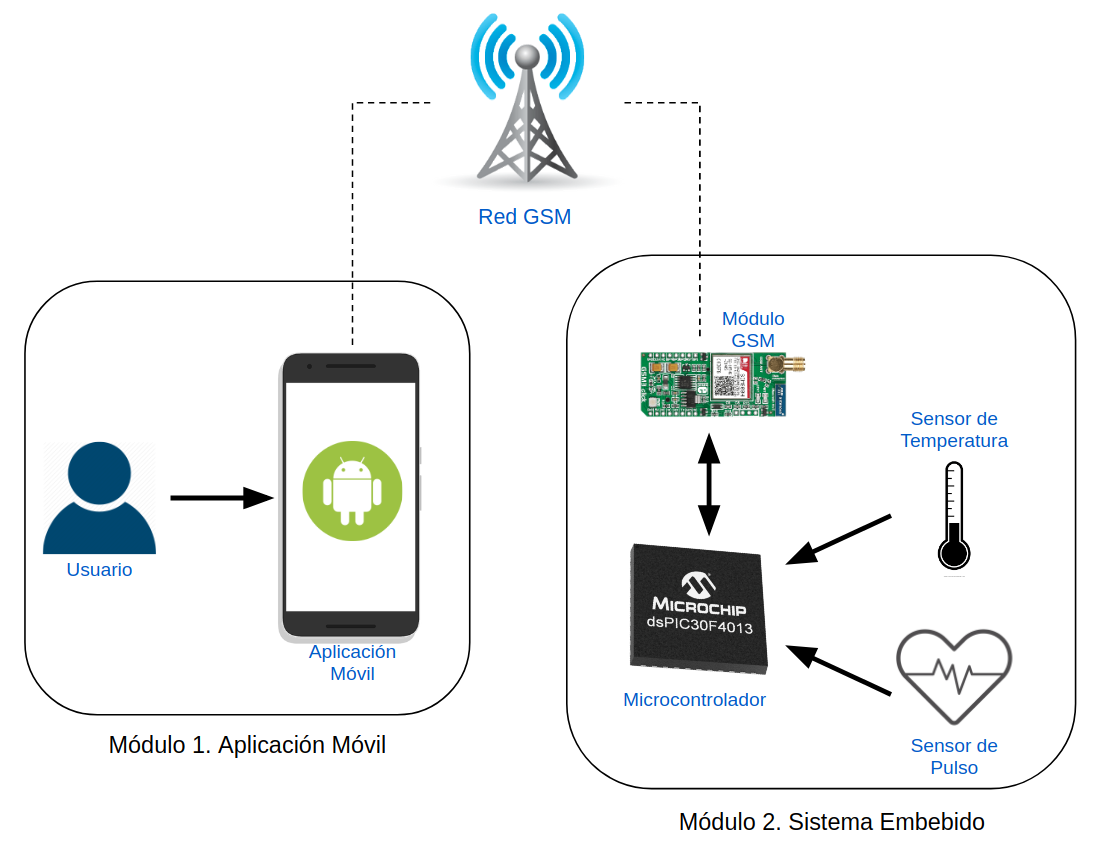
\includegraphics[width=0.9\textwidth]{DisenoEstructura/imagenes/arquifisica.png}}
	\caption{Arquitectura física del sistema}
	\label{fig:DisenoArquiFisica}
\end{figure}

\section{Arquitectura lógica del sistema}
En la figura \ref{fig:DisenoArquiLogica} se muestra la arquitectura lógica del sistema, la cual describe de forma más específica el funcionamiento de los módulos en conjunto para su correcto funcionamiento.\\



\begin{figure}[htbp!]
	\centering
	\fbox{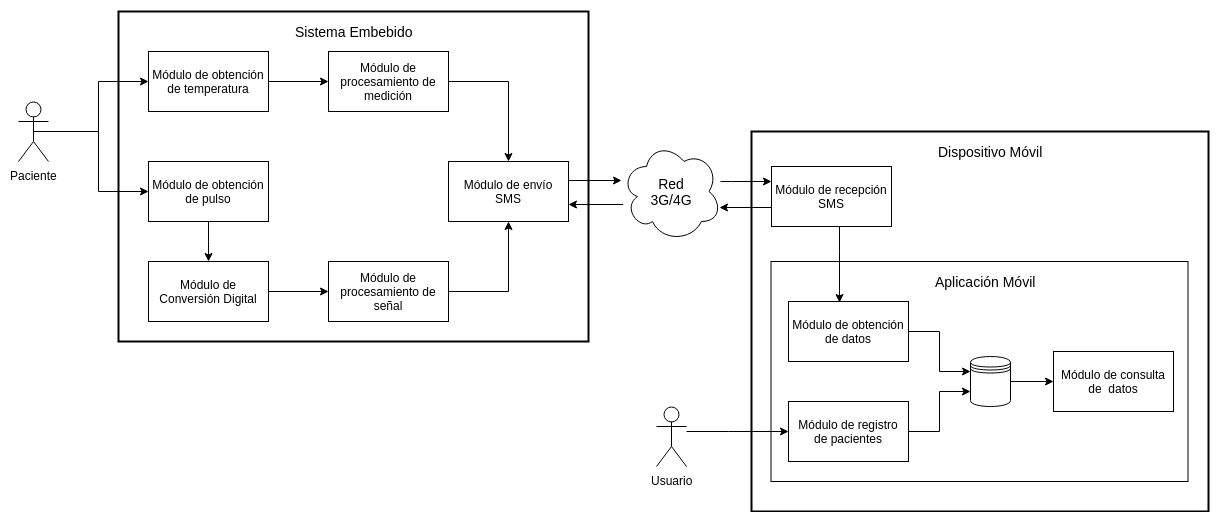
\includegraphics[width=0.9\textwidth]{DisenoEstructura/imagenes/arquitectura.png}}
	\caption{Arquitectura lógica del sistema}
	\label{fig:DisenoArquiLogica}
\end{figure}